\section{Approaching the five-dimensional case}
\noindent Due to time constraints our research into the five-dimensional case has been rather sparse. However, our formalization of the problem and the theoretical framework introduced does enable us to provide a few insights. We begin with a RDTS.

\begin{example}[RDTS for $n = 5$]\label[example]{ex:5d-rdts}
In this case all overlap inequalities have arity $1$, $2$, $3$ or $4$. By \cref{prop:arity-reduction} we only have to consider the overlap inequalities with arity $1$ or $2$. We would like to choose a dimension tuple $\paren{x_1, x_2, x_3, x_4, x_5}$ satisfying Hoffman's inequality and containing distinct elements, since by doing so we can make sure that of the overlap inequalities with arity $1$, such a dimension tuple will only satisfy the trivial ones. Then we only need to consider the overlap inequalities with arity $2$. Next, we follow the same line of thought as in \cref{ex:4d-rdts} where it resulted in a pair of non-trivial overlap inequalities, where at most one could not be satisfied. This resulted in an RDTS with two dimension tuples. Now, we end up with 5 pairs, namely 
\begin{align*}
\paren{A, B}, \paren{B, A}, 
&\paren{B, C}, \paren{C, B},\\
\paren{C, D}, \paren{D, C}, 
&\paren{C, F}, \paren{C, F},\\
\paren{E, F}, & \paren{F, E},
\end{align*}
where
$A = \curly{1, 4}$, 
$B = \curly{2, 3}$, 
$C = \curly{1, 5}$, 
$D = \curly{2, 4}$, 
$E = \curly{2, 5}$
and
$F = \curly{3, 4}$. Hence, any dimension tuple must always satisfy at least five non-trivial overlap inequalities. Intuitively, we are attempting to cover every possible way to linearly order the sums of two distinct terms (without any two sums with different terms being equal) and this is illustrated in \cref{fig:hasse-5d-arity-2}. Then, one might suspect there to be $2^5 = 32$ minimal equivalence classes of dimension tuples, but this is not the case. Some of these overlap inequalities are in fact mutually dependent on one another in an intricate way as illustrated in \cref{fig:5d-decision-tree}.
\begin{figure}[ht]
    \centering
    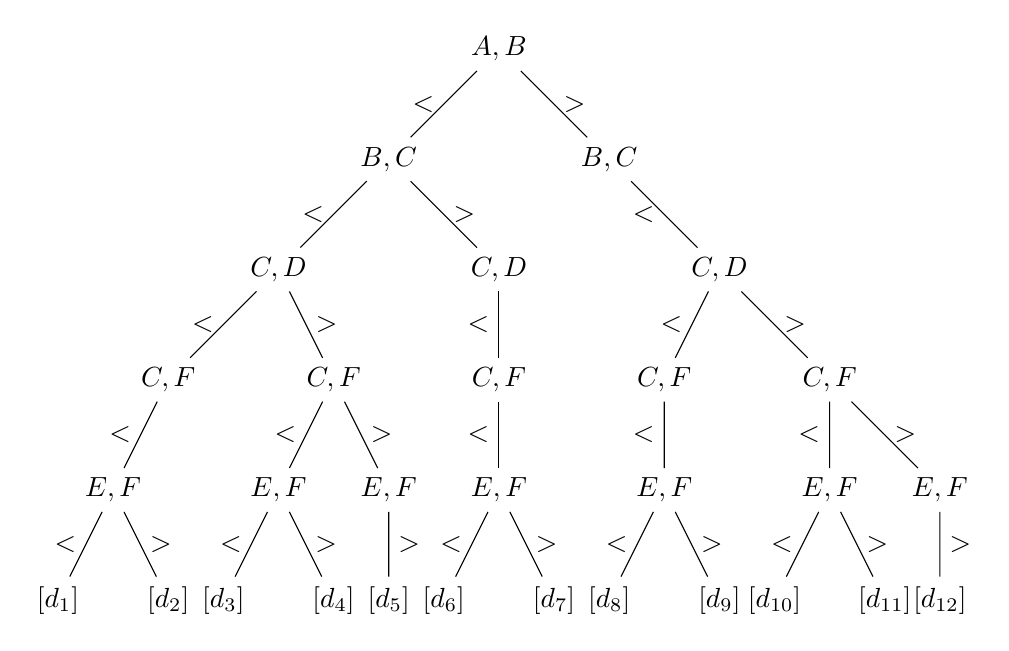
\begin{tikzpicture}[scale=0.70]
        \node(d1) at (-8, 0) {$[d_1]$};
        \node(d2) at (-6, 0) {$[d_2]$};
        \node(d3) at (-5, 0) {$[d_3]$};
        \node(d4) at (-3, 0) {$[d_4]$};
        \node(d5) at (-2, 0) {$[d_5]$};
        
        \node(d6) at (-1, 0) {$[d_6]$};
        \node(d7) at (1, 0) {$[d_7]$};
        
        \node(d8) at (2, 0) {$[d_8]$};
        \node(d9) at (4, 0) {$[d_9]$};
        \node(d10) at (5, 0) {$[d_{10}]$};
        \node(d11) at (7, 0) {$[d_{11}]$};
        \node(d12) at (8, 0) {$[d_{12}]$};
        % (E, F)
        \node(ef1) at (-7, 2) {$\paren{E, F}$};
        \node(ef2) at (-4, 2) {$\paren{E, F}$};
        \node(ef3) at (-2, 2) {$\paren{E, F}$};
        \node(ef4) at (0, 2) {$\paren{E, F}$};
        \node(ef5) at (3, 2) {$\paren{E, F}$};
        \node(ef6) at (6, 2) {$\paren{E, F}$};
        \node(ef7) at (8, 2) {$\paren{E, F}$};
        % (C, F)
        \node(cf1) at (-6, 4) {$\paren{C, F}$};
        \node(cf2) at (-3, 4) {$\paren{C, F}$};
        \node(cf3) at (0, 4) {$\paren{C, F}$};
        \node(cf4) at (3, 4) {$\paren{C, F}$};
        \node(cf5) at (6, 4) {$\paren{C, F}$};
        % (C, D)
        \node(cd1) at (-4, 6) {$\paren{C, D}$};
        \node(cd2) at (0, 6) {$\paren{C, D}$};
        \node(cd3) at (4, 6) {$\paren{C, D}$};
        % (B, C)
        \node(bc1) at (-2, 8) {$\paren{B, C}$};
        \node(bc2) at (2, 8) {$\paren{B, C}$};
        % (A, B)
        \node(ab) at (0, 10) {$\paren{A, B}$};
        
        % Layer 0-2
        \draw (ef1) -- (d1) node [midway, left] {$<$};
        \draw (ef1) -- (d2) node [midway, right] {$>$};
        \draw (ef2) -- (d3) node [midway, left] {$<$};
        \draw (ef2) -- (d4) node [midway, right] {$>$};
        \draw (ef3) -- (d5) node [midway, right] {$>$};
        
        \draw (ef4) -- (d6) node [midway, left] {$<$};
        \draw (ef4) -- (d7) node [midway, right] {$>$};
        
        \draw (ef5) -- (d8) node [midway, left] {$<$};
        \draw (ef5) -- (d9) node [midway, right] {$>$};
        \draw (ef6) -- (d10) node [midway, left] {$<$};
        \draw (ef6) -- (d11) node [midway, right] {$>$};
        \draw (ef7) -- (d12) node [midway, right] {$>$};
        
        % Layer 2-4
        \draw (cf1) -- (ef1) node [midway, left] {$<$};
        
        \draw (cf2) -- (ef2) node [midway, left] {$<$};
        \draw (cf2) -- (ef3) node [midway, right] {$>$};
        
        \draw (cf3) -- (ef4) node [midway, left] {$<$};
        
        \draw (cf4) -- (ef5) node [midway, left] {$<$};

        \draw (cf5) -- (ef6) node [midway, left] {$<$};
        \draw (cf5) -- (ef7) node [midway, right] {$>$};
        
        % Layer 4-6
        \draw (cd1) -- (cf1) node [midway, left] {$<$};
        \draw (cd1) -- (cf2) node [midway, right] {$>$};
        
        \draw (cd2) -- (cf3) node [midway, left] {$<$};
        
        \draw (cd3) -- (cf4) node [midway, left] {$<$};
        \draw (cd3) -- (cf5) node [midway, right] {$>$};
        
        % Layer 6-8
        \draw (bc1) -- (cd1) node [midway, left] {$<$};
        \draw (bc1) -- (cd2) node [midway, right] {$>$};
        
        \draw (bc2) -- (cd3) node [midway, left] {$<$};
        
        % Layer 8-10
        \draw (ab) -- (bc1) node [midway, left] {$<$};
        \draw (ab) -- (bc2) node [midway, right] {$>$};
    \end{tikzpicture}
    \caption{Decision tree showing how not satisfying certain overlap inequalities affect other overlap inequalities. It is quite helpful to compare this with \cref{fig:hasse-5d-arity-2}.}.
    \label{fig:5d-decision-tree}
\end{figure}
By looking at this decision tree we observe that there are in reality only 12 minimal elements. For each of these we have found a representative satisfying Hoffman's inequality, namely
\[
\begin{aligned}[c]
d_1 &= \paren{28, 31, 34, 36, 38},\\
d_4 &= \paren{20, 22, 24, 25, 28},\\
d_7 &= \paren{24, 28, 29, 30, 32},\\
d_{10} &= \paren{20, 21, 24, 26, 28},
\end{aligned}
\quad
\begin{aligned}[c]
d_2 &= \paren{22, 25, 26, 28, 30},\\
d_5 &= \paren{18, 20, 21, 22, 26},\\
d_8 &= \paren{22, 24, 26, 29, 30},\\
d_{11} &= \paren{24, 26, 28, 31, 34},
\end{aligned}
\quad
\begin{aligned}[c]
d_3 &= \paren{26, 28, 32, 33, 36},\\
d_6 &= \paren{22, 25, 27, 28, 29},\\
d_9 &= \paren{26, 29, 30, 34, 36},\\
d_{12} &= \paren{15, 16, 17, 19, 22}.
\end{aligned}
\]
Hence, the set of these 12 dimension tuples constitutes a RDTS for $n = 5$.
\end{example}

\noindent In the four-dimensional case we immediately began counting the number of unique universal packings, since 4 is a good dimension by \cref{thm:multiplication-of-packings}. However, we do not know whether 5 is a good dimension and whether a universal packing exists. Until then we might be better off trying to find a Hoffman packing of each of these 12 dimension tuples individually. Intuitively, they represent the 12 most difficult types of dimension tuples to solve.

\begin{remark}
What about the criteria found to be necessary properties of universal packings? Interestingly, each of the 12 dimension tuples above has properties similar to those of the dimension tuple in \cref{lemma:finding-tuples}, whereby any Hoffman packing of it must necessarily satisfy the Line criterion \labelcref{criterion:line-criterion}. Then the Subgrid criterion \labelcref{criterion:subgrid-criterion} must hold as well. In fact, we suspect that in higher dimensions minimal equivalence classes of dimension tuples will always result in any Hoffman packing necessarily satisfying the Line criterion \labelcref{criterion:line-criterion}.
\end{remark}

\noindent 

\noindent Next, we highlight a few investigations which we deem particularly interesting. They have not been pursued further due to time constraints.

\subsection{Fundamentally different approaches}
It would be interesting to explore the possibilities of making ``local changes'' to a pseudo-packing and use this to gradually reduce the number of overlapping hyperrectangles. One could begin by further exploring the results obtained in \cref{obs:3d-distances}.

It would also be interesting to explore the possibility of reducing a higher dimensional packing to a packing in lower dimensions. This would enable us to create a five-dimensional packing via a reduction of a six-dimensional one obtained via \cref{thm:multiplication-of-packings}. We have made a few failed attempts at reducing a four-dimensional packing to a three-dimensional one. However, others might have better luck.

\subsection{Ties to Maclaurin's inequality}
There are a number of ways to further explore the results obtained in \cref{obs:4d-n-2-subgrid}. First of all, it would be interesting to see if imposing such a criterion significantly speeds up the search process in the four-dimensional case. It is unclear whether this might be the case, since the Subgrid criterion \labelcref{criterion:subgrid-criterion} has proven quite effective at pruning the search tree in the three-dimensional case (as seen in \cref{fig:backtracking-3d}), but less effective in the four-dimensional case (as seen in \cref{fig:backtracking-4d}).

Note that it is still relevant to look for four-dimensional universal packings through other approaches in order to explore whether such a criterion is a necessary condition for being a universal packing.

We suspect that it might also be possible to put forward similar criteria for the five-dimensional case by looking at Maclaurin's inequality for $n = 5$. A way to better justify imposing such rather speculative constraints would be to construct a six-dimensional universal packing by combining a two- and a three-dimensional universal packing and then examining whether it exhibits similar criteria for $n = 6$.

\subsection{Formulation as a constraint satisfaction problem}
\noindent During the course of this project, it has become increasingly clear that it is most natural to formulate Hoffman's multidimensional packing problem as a constraint satisfaction problem (CSP). This class of problems has been subject to intense research in both artificial intelligence and operations research and one will thus be able to draw upon the advances in these fields. A CSP as described in \cite{CSP1999} and \cite{bartak1998} consists of a list of variables, a list of their respective value domains and a set of constraints over the variables. Then a solution is a choice of a value for each variable such that all constraints are satisfied. When solving a CSP we can look for one or all solutions and this corresponds perfectly to the types of questions raised about our packing problem.

The most common search algorithm for solving CSPs is backtracking, and here there are several ways to tune it, including the order in which variables are assigned values as well as the order in which compatible values are chosen.

For instance, one could employ a dynamic variable ordering in which the choice of the next variable to be assigned a value depends on the current state of the search. It is a common heuristic to select the variable with the fewest remaining compatible values. If the current partial solution can be completed to a solution, then every remaining variable must be assigned a value. The variable with the smallest domain is likely to be the most difficult to find a value for, since assigning values to other variables first may further reduce the number of compatible values.

Next, the order in which the values are tried out can also be adjusted. A different value ordering will rearrange the branches springing from each node of the search tree. This is an advantage if it results in searching a branch leading to a solution earlier than branches leading to dead ends. For instance, if a CSP has a solution and if a correct value is chosen for each variable, then a solution can be found without any backtracking.

Hence, formulating the problem as a CSP might enable us to prune the search tree thoroughly and let us experiment with finding the best variable ordering and value ordering. In retrospect the approaches tried out in this project may actually be thought of as immature variants of such a backtracking algorithm.

The backtracking approach presented earlier places one hyperrectangle at a time. However, a CSP solver might only specify some of the extends of a hyperrectangle and wait with the rest until later. It will also have more opportunities to experiment with variable ordering, whereas we could only place hyperrectangles on top of those already placed.

The dynamic programming approach can also be analyzed within this framework. It is really a search for gradually larger groups of mutually compatible assignments of values. Take for instance the case of constructing a cube by stacking squares. Here the constraints only related to the assigned square will always be satisfied. However, this analysis also reveals a weakness of the approach. Not only does it need a large amount of memory to store the mutually comparable values (e.g. all squares), it is also very questionable whether this variable ordering is the most effective. In particular, this consideration shows why it might not be helpful to combine for instance orthogonal squares. One would assign values to many variables with untouched domains, while possibly ignoring variables with very few compatible values left.

We speculate that a formulation as a CSP might be well-suited for searching for a four-dimensional universal packing and perhaps even attempt to determine the number of unique cubes in the four-dimensional case, where one should also be able to parallelize the search by dividing the problem into smaller parts using kernels.

With assistance from Trine K. Boomsma, we approached the packing problem using mixed-integer programming. This approach turned out to be ill-suited, since the search algorithms spent a lot of time looking for non-optimal solutions, while we are really only interested in optimal integer solutions. However, exploring this field made it more clear that approaching the problem using constraint satisfaction is well worth a try. We suspect that existing general purpose CSP solvers (commercial as well as free ones) are not flexible enough to take full advantage of the domain-specific knowledge of this problem. In particular, we fear that solving simultaneously for multiple dimension tuples (such as those in a RDTS) might not be possible. Also, we fear that constraints imposed by results obtained by investigations into the links to Maclaurin's inequality might be difficult to express. Hence, a custom implementation of a CSP solver might be worth looking into.
